\documentclass[a4paper,norsk]{article}
\usepackage{preamble}

\begin{document}
\maketitle

\section*{Exercise 1}
\subsection*{a}
\begin{figure}[h!]  
  \centering
  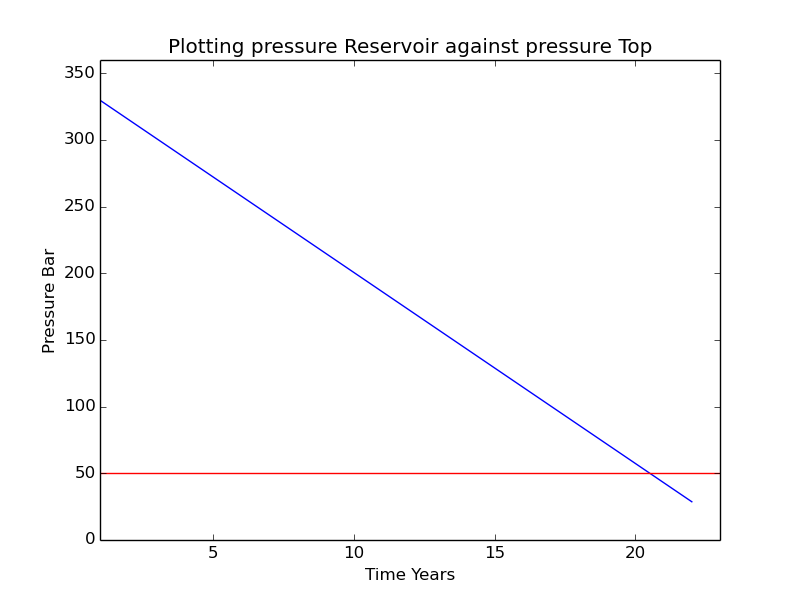
\includegraphics[scale=0.4]{Pressure.png}
\end{figure}
This figure presents the theoretical pressure at the recieving end onshore. From the proposed production profile I have assumed  
\begin{itemize}
\item linear pressure drop of 15 bar per year
\item From mass flow calculated the velocity \textit{u} to be 9m/s in the wellpipe, and 3.5 m/s in the export pipe. Using
\begin{align}
U = \frac{4Q}{\rho \pi D^2}
\end{align}
\end{itemize}
Using the assumptions presented in the exercises, my computations results in a pressure beneath the critical value 50 bar at 21 years.


\subsection*{b}
So according to my answer in exercise a, pressure support is necessary after 21 years of production.
\subsection*{c}
The fact that the contribution of liquid is neglected in this multiphase flow is due to a high Gas Oil Ratio (GOR), larger than 40000. In other words gas is dominating in the flow. The main uncertainties of this approximation is the fact that in multiphase flow the fluids contribute more to a pressuredrop  than gas. Because of higher density we might get a lower pressuredrop in the calculations compared to the reality. Another contribution to error is the approximation of constant density, which is not the fact to a gas dominated flow which is compressible.

\subsection*{d}
To improve the pressure drop calculations we might consider to use a more advance model, which of course will result in more complexity. Firstly using a constant density through the pipesegment results in poor results, due to the fact that we operate with compressible hydrocarbons. We also neglect the path of the pipes, assuming 1D calculations which will not be able to catch the physical influence from the geometry and path of the pipes. Also setting the dynamic viscosity constant for such a system will also degrade the quality of the calculations. Summed up the assumptions of constant contributions from the physics and geometry will result in inexact results. To improve the calculations we have to include change of parameters, which will of course make the calculations more complex. 

\subsection*{f}
Choosing subsea compression auxiliary systems are necessary to protect the equipment and maintain an efficient production rate.
\begin{itemize}
\item Slugging is a threat to the compressor and its interior. Installing an inlet separator prior to the compressor ensures that the compressor only handles clear phases, and not any solids.
\item Reducing liquid droplets in the compressor suction is essential to preserve the compressor. This is often called liquid carry over, and can be opposed by using a scrubber which is a system designed to remove these liquid droplets from the gas stream.
The reason these liquid droplets pose a risk is at the present liquids such as water and in some sense oil is incompressible. To much incompressible vapor will damage the compressor piston as it strikes, and can overtime give extensive damage to the compressor
\item Sediments pose a risk aswell which will damage the compressor parts if they are not taken out of the gas stream. To help out reduce these sediments, chemicals can be added further down the stream to decompose the sediments before they reach the compressor inlet.
\end{itemize}

\subsection*{g}
Choosing a topside or a subsea compression presents different development impacts. \\
\textbf{Project execution} \\
Firstly looking at production point of view a subsea solution is more efficient to produce. A topside compressor demands a platform where it can be operated, and personnel to man the platform. A subsea solution demands neither, resulting in a lot of cost savings. \\
Aker solutions have also calculated a reduced CO2 emission of 60\% due to the fact that the requirement of a platform is no longer essential. 

\textbf{Operation} \\
Even though both solutions are made do operate for long periods of time, incidents happen. A compressor located on a platform is easier and more cost efficient to maintain in operation, while a subseacomponent needed to be changed is very expensive. On the other hand a subsea solution is not exposed to harsh weather and ice found accordingly in tropic and artic areas, while a rig operation can be delayed by these factor due to equipment and personel safety. \\
Production over time will reduce the wellhead pressure, resulting in decreased flowrate in the pipes to the production site. Using a compressor subsea will increase productionrate by reducing the backpressure at the well as reservoir pressure is reduced over time. The pipes from the well often travels several thousand meters before they reach a topside compressor, and therefore this solution cannot give such a instant effect on the reservoir as a subsea solution.

\subsection*{h}
Installing a subsea compressor from day 1 will from my calculations increase the available production time with 3-4 years. Of course an installment of the compressor at startup will increase the cost at that time. However with an expectaoncy 3-4 years of production, even with lower volumes of hydrocarbons, will make up for that as a longtime investment.



\section*{Exercise 2}
In this section will will look at at the following flow assurance issues
\begin{itemize}
\item Wax
\item Hydrates
\item Slug
\end{itemize}

\subsection*{a}
The presented figures are the calculated temperatures in the pipe system. The first figure represents 
\begin{figure}[h!]  
  \centering
  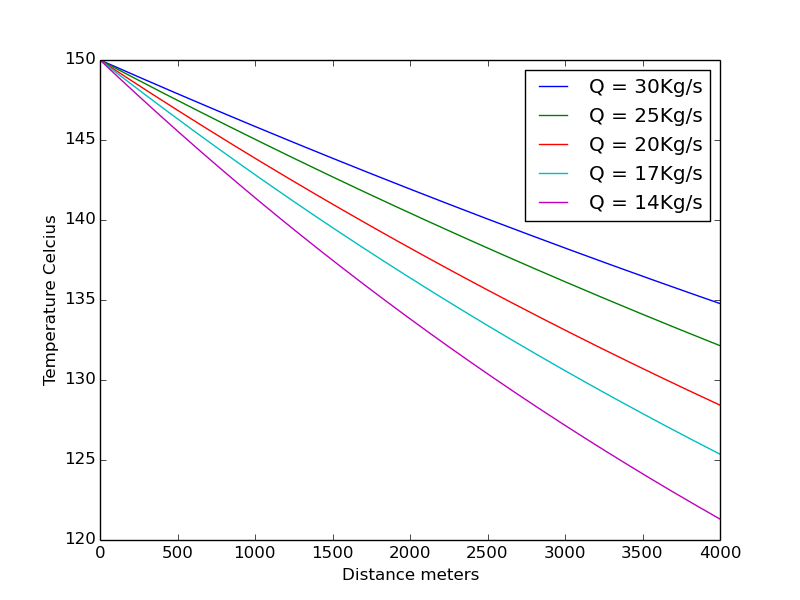
\includegraphics[scale=0.4]{wellhead.png}
  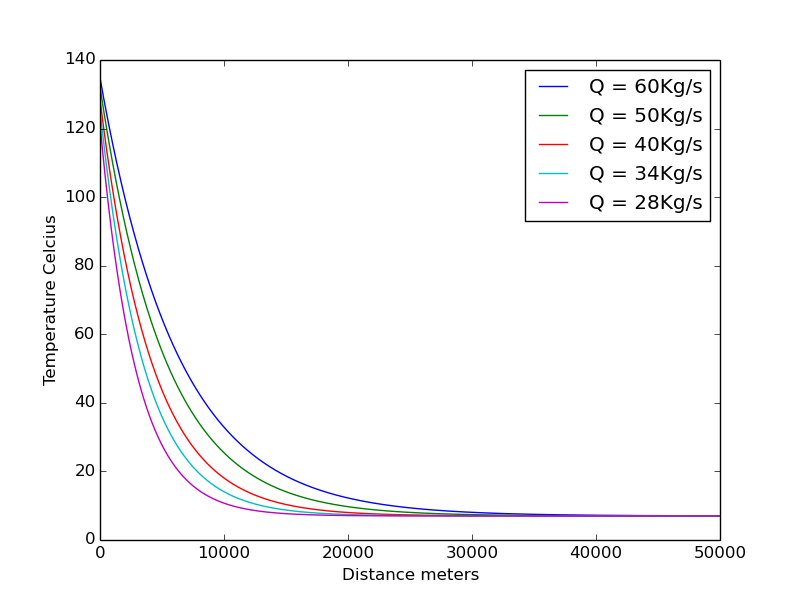
\includegraphics[scale=0.4]{shore.png}
\end{figure}
\newpage

\subsection*{b}
From our lecture notes we know the following conditions are required to form hydrates
\begin{itemize}
\item High pressure: typically above 10-20bar at ambient temperature
\item Low temperatures: typically below 20-25 Celcius.
\end{itemize}
Looking at our temperature profiles we observe that for the flow from the reservoir to the well, we operate within feasible temperatures. For the pipeline from the well to shore, the temperature will eventually drop beneath this critical of 20 Celcius due to the long time of low seatemperature exposure. Different preventative measures can be taken to keep hydrates out of the system, discussed in \textit{exercise 3}

\subsection*{c}
From our pressure profile for each year and corresponding temperature profile, we will unfortunately fall below the
Wax appearance temperature (WAT) presented in Figure 4 in the exercises. Especially critical around 10 years, our pressure will be around 220 bar which has a peak on the WAT chart. This means that our gasflow will for a longer time be exposed to critical temperatures below WAT, resulting in a higher risk of wax deposits in the pipe. This will occur in the pipeline from the wellhead to shore. Regular pigging of the pipe may contribute to keep the risk of wax plugs low. Other measures can be used to manipulate WAT in gas flow, such as separation at different temperatures. 

\section*{Exercise 3}
As stated in the lecture notes hydrate management philosophy is field specific. From field to field different retarding factors influence the theoretical hydrate equilibrium conditions, but the main goal for all fields is to stay outside the hydrate formation envelope calculated by these factors. \\
One most consider how to handle hydrates in normal operation as well as during and under the recovery of system shutdowns. Hydrates are formed when light hydrocarbon molecules and water are present under certain pressure and temperature conditions. Our strategy must include active measures to counter these conditions to happen in our system.  
Our system operates with a high GOR, we can use control measures such as 
\begin{itemize}
\item \textbf{Water removal} \\
Liquid water is an essential part of hydrate formations to occur. By dehydrating the gasflow to a certain water dew-point we can prevent the creation of hydrate formations for the specific system.

\item \textbf{Chemical injection}
Chemical injection can be used to alter the conditions for hydrates forming as well as their structure. \\
\textit{Thermodynamic inhibitors} are used to lower the hydrate equilibrium temperature which formations can be formed, resulting in that the gasflow can handle lower temperatures without hydrates beeing formed. \\
\textit{Low-concentration inhibitors} are used to alter the hydrate structure delaying the hydrate or making them unable to plugg the line.

\item \textbf{Compression}
For a gas dominating system which is offline, one can increase the temperature by compressing the hydrocarbons before a restart which will increase the temperature. This will help keeping the hydrocarbons outside the temperature needed where hydrates can exist. 
\end{itemize}

\newpage
\section*{Exercise 4}
\begin{figure}[h!]  
  \centering
  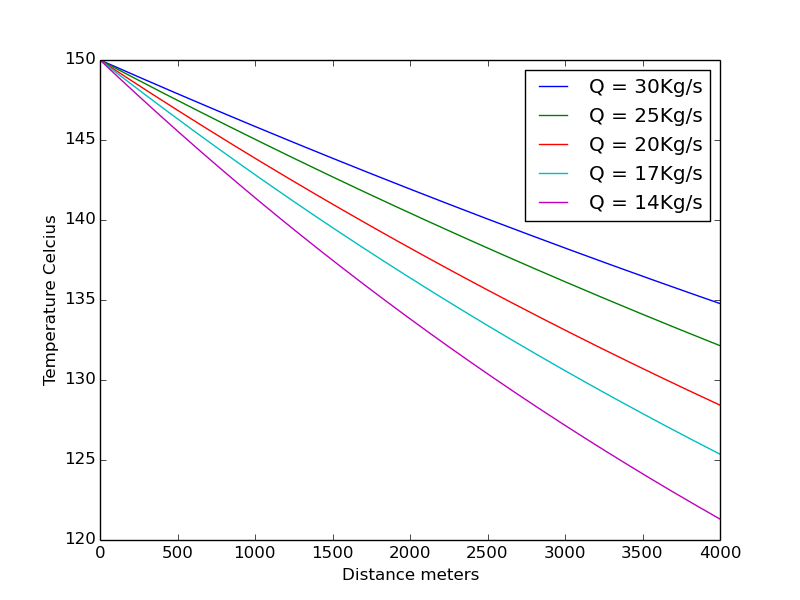
\includegraphics[scale=0.4]{TASK4wellhead.png}
  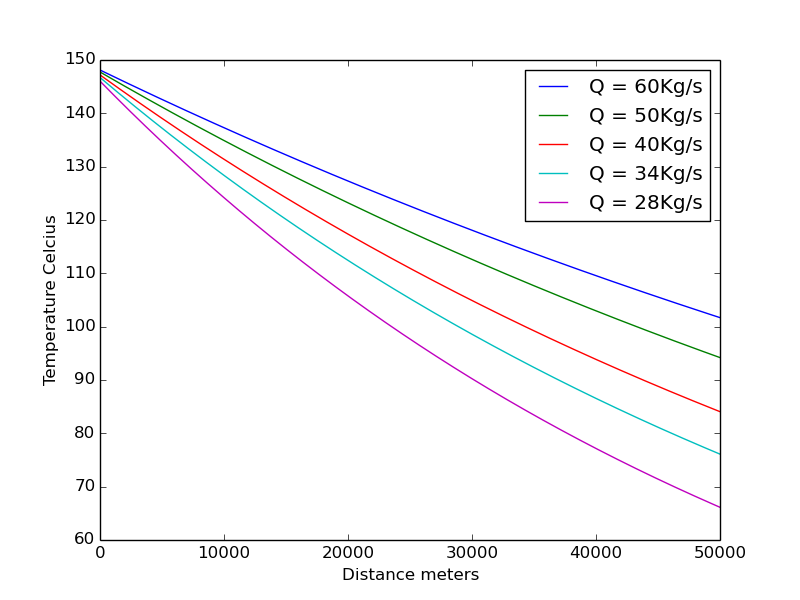
\includegraphics[scale=0.4]{TASK4shore.png}
\end{figure}
Using a pipeline with Uvalue as 1, we observe some drastic results. The change in insulation results in a mutch lower temperaturedrop in both pipesections. We observe that in the first pipeline temperature will stay over 145 Celcius for a flow properties of Q. While for the second pipelinesecion to shore, the temperatue will stay within 70-100 Celcius depending on Q. \\
This yields positive results for the wax and hydrate management. The insulation will keep the fluid temperatures above hydrate equilibrium temperatures, resulting for minimum risk of hydrates forming in the flow. This also contributes to reducing the creation of wax, due to the fact that the insulation will help keep the temperature above wax appearance temperature (WAT)


\newpage
\section*{Exercise 5}
During X-mas tree design we have to be aware of both internal and external flow, which can force mechanical vibrations from pressure oscillations. This becomes dangerous if the oscillations hits one of the system eigenfrequencies. External flow from local current can produce these oscillations around a pipesegment due to vortexes created by the geometry. \\
For flow-induced vibrations in the pipeline, resonance cannot be avoided. Due to the fact that flow excitation is able to reach a wide range of frequencies, we cannot avoid resonance by trying to change the eigenfrequencies of our tree. Therefore weak spots have to be reinforced so that the estimated time before a failure occurs is longer than the production lifetime. This can be simulated using Computational Fluid Dynamics, and analysis in structural mechanics. \\
It is worth to mention that acoustic pulsation in dead legs can cause pressure oscillations if the vortex shedding from these dead legs is the same as one of the acoustic frequencies of the dead leg. As I interpret the question this is not a flow induced vibration, but is worth mentioned.

\subsection*{Subsea design and development}
Different factors have influence of the development solution. 

First and foremost we have to know what hydrocarbons we are going to produce. We also need to know the length of the well to reach the reservoir,, which may be several thousand meters. Overtime this might require pumps ,compressors and waterinjection to maintain pressure for production. 
A larger reservoir requires more productiontrees if we want to exploit the reservoir for maximum production. 
The amount of production trees and manifolds lay basis for the amount of powersupply needed to maintain operation, as well as supporting unit such as compressors, pumps and separators. \\


These factors imply that for each productiontree we need support units to help maintain production.
\begin{itemize}

\item \textbf{Separation}
 Firstly all producing X-mas trees run their production into a separator. Here the production is separated from water and hydrocarbons. The gas and oil are also separated, so the gas can be compressed before they are sent in the export pipe.
\item \textbf{Injection}
Close to the wellheads waterinjection templates are installed which pumps the water back in the reservoir to maintain the pressure and productionrate.

\item{Cooling}
Cooling manifolds may be needed depending on the field, to cool down the flow before entering other production system. This is simply because some units might not be able to handle the high temperatures. 

\item \textbf{Power and Control}
A main controlbase are built to distribute electrical power and control the whole subsea section. Here the whole production is monitored from personnel on a production ship or a on land. \\
\item \textbf{Distances}
Factors such as water depth and distance to the receiving end of the export pipeline, will influence the amount of pumps, compressors and electrical power to power the transport of hydrocarbons from the subsea factory. This will result in more subsea components needed to be built. \\
Due to norwegian law, each subsea unit must be protected by a 
welded metalroof to protect the units from fishing operations and subsea debris. \\ 
\item \textbf{ROV}
One might also consider to lay all pipes and wires needed for production on the seabed, to make ROV operations safe and to avoid the chance of damages on the system while operating the ROV.
\end{itemize}



\section*{Exercise 6}
The main property of a subsea Christmas tree is to control the flow of hydrocarbons from the well and to the production recipient. It is placed directly ontop the wellhead,and some of the main functions are

\begin{itemize}
\item \textbf{Flow} \\
With a number of chokes and valves in the X-mas tree design, the tree is able to control the rate of flow of hydrocarbons as well as control and balance pressure in the system. The tree doesn't only control vales and chokes within itself, but also furhter down in the wellpipes. \\The X-mas tree is also equipped with a safety design in the mastervalves. In case of a powercut, these vales which are maintained open by hydraulics will close automatically and stay closed until the failure has been assesed and the system restarted. The tree is alos equipped with pressurevalves, to control and relive pressure in case it gets higher than the system specification.

\item \textbf{Injection points} \\
Used to inject chemicals into the flow, which is important to reduce the possibility wax and hydrates building up in the system, retarding the operation. This is included in the X-mas design so that the injection can be done in the X-mas tree or further downhole.

\item \textbf{Well intervention} \\
And important functionality to operate downhole vales, lower measurement equipment, regular maintenance and pigging operations. The X-mas tree is desiged such that these interventions are often done through the topside valve often called swab valve. 
\item \textbf{Monitoring} \\
The X-mas tree is equipped with several monitoring systems overlooking vital data such as pressure, temperature, flow composition, erosion and flow induced vibrations. This is registered within the tree through internal sensors within the tree, distributed in several section in the tree so if one sensor fails, another can give accurate measurements.
\end{itemize}

\begin{figure}[h!]  
  \centering
  \caption{X-mas Tree}
  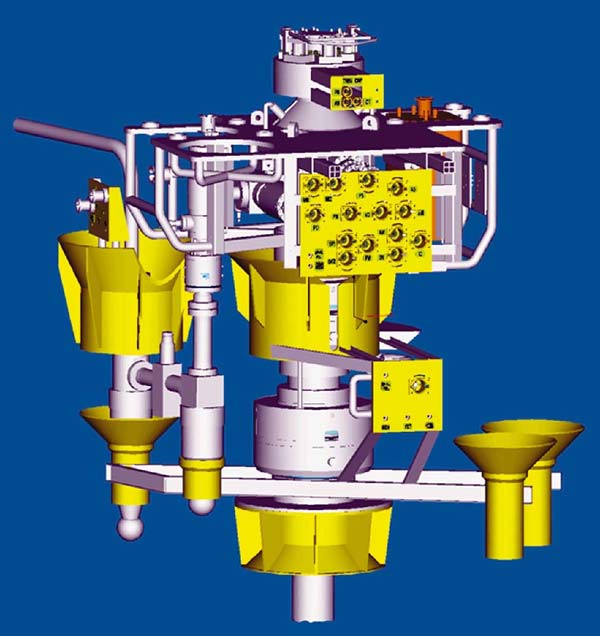
\includegraphics[scale=0.4]{xmas.jpg}
\end{figure}





\end{document}
